\section{Neural Network Based Signal Selection}
\label{sec:hh_strategy}

%%%%%%%%%%%%%%%%%%%%%%%%%%%%%%%%%%%%%%%%%%%%%%%%%%%%%%%%%%%%%%%%%%%%%%%%%%%%%%%%%%%
%%%%%%%%%%%%%%%%%%%%%%%%%%%%%%%%%%%%%%%%%%%%%%%%%%%%%%%%%%%%%%%%%%%%%%%%%%%%%%%%%%%
%%%%%%%%%%%%%%%%%%%%%%%%%%%%%%%%%%%%%%%%%%%%%%%%%%%%%%%%%%%%%%%%%%%%%%%%%%%%%%%%%%%
%
% NN 
%
%%%%%%%%%%%%%%%%%%%%%%%%%%%%%%%%%%%%%%%%%%%%%%%%%%%%%%%%%%%%%%%%%%%%%%%%%%%%%%%%%%%
%%%%%%%%%%%%%%%%%%%%%%%%%%%%%%%%%%%%%%%%%%%%%%%%%%%%%%%%%%%%%%%%%%%%%%%%%%%%%%%%%%%
%%%%%%%%%%%%%%%%%%%%%%%%%%%%%%%%%%%%%%%%%%%%%%%%%%%%%%%%%%%%%%%%%%%%%%%%%%%%%%%%%%%


The current analysis makes use of a multi-output classifier, one that does not simply classify
a single process against a single background label, but rather a classifier that provides multiple
output labels with each pertaining to a distinct class or process.
One of the easiest ways to build such a classifier is to take a multi-variate approach that
is by default suitable for multi-output classification: neural networks.

\subsection{Classifier Architecture}
\label{sec:nn_arch}

The analysis makes use of a deep-learning, neural network based approach.
The classifiers that we build are trained to classify $pp$ collision events according to
four potential class labels, inspired by the dominant expected background processes:
\begin{enumerate}
    \item Dilepton non-resonant $hh \rightarrow \bbww$
    \item SM top-quark processes ($\ttbar + Wt$), `Top'
    \item SM $Z$+jets processes, $Z \rightarrow \{ee,\mu\mu\}$
    \item SM $Z$+jets processes, $Z \rightarrow \tau\tau$
\end{enumerate}
The classifier is trained with separate labels for the $Z \rightarrow \{ee,\mu\mu\}$ and
$Z \rightarrow \tau\tau$ processes as these lead to clearly different final state kinematics.
The dilepton final state that we eventually select in the analysis is composed only of electrons and/or muons.
The $Z \rightarrow \tau\tau$ process contributes only in the cases where both $\tau$ leptons decay
leptonically.
The electrons and muons from these $\tau$ decays have very different kinematic signatures as compared
to those from the direct decays of the $Z$-bosons.
Allowing the classifier to learn how to distinguish between these $Z$ decays improves its overall performance
to separate the $hh$ signal process from the backgrounds.

We construct the neural network architecture using the \textsc{Keras}~\cite{chollet2015keras}
library, using \textsc{Tensorflow}~\cite{tensorflow2015} as a backend.
An illustration of the neural network architecture is given in Figure~\ref{fig:nn_arch}.
The network inputs are passed through a dense (fully-connected) layer,  which
is trained with a dropout layer, and then a second dense layer.
The final activation is a softmax activation~\cite{GoodFellowBook}.

\begin{figure}[!htb]
    \begin{center}
        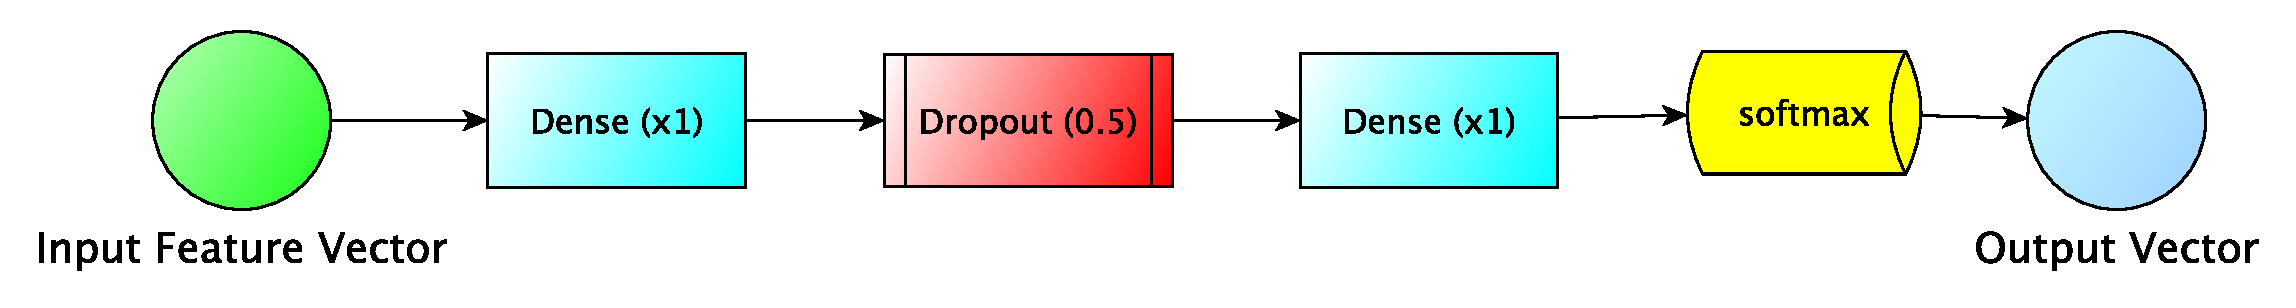
\includegraphics[width=0.85\textwidth]{figures/search_hh/mva/nn_arch_graph_updated}
        \caption{
            Illustration of the neural network graph employed in the analysis.
            The input feature vector has a length of 35 and the output vector is length 4,
            one for each of the targeted processes.
        }
        \label{fig:nn_arch}
    \end{center}
\end{figure}
Each of the dense layers are 250 nodes wide and  have their weights randomly initialized by sampling
from a truncated normal distribution centered on zero with a width given by $\sqrt{1/N_{\text{inputs}}}$, where
$N_{\text{inputs}}$ is the number of input features (the length of the input vector).
The activation functions for each of the dense layers are rectified linear units (`ReLu')~\cite{ReLu}.

Using an output layer with a softmax activation function allows one to interpret the outputs as
each representing a probability\footnote{
The use of the term `probability' here is not entirely correct, as the outputs are not \textit{strictly} probabilities given the fact that the network
does not know about the full set of possible processes that will be presented to it when it is used outside
of the training stage and in the analysis.
This is clear from the fact that the sum appearing in the denominator of Equation~\ref{eq:softmax_activation}
is not over the full set of processes that will be provided as input to the network when it is used
in the analysis.
The sum is only over those processes that we have decided to train the classifier to provide labels for.
Additionally, the labelled
processes are presented in artificial proportions during the training process, described in Section~\ref{sec:nn_train},
which may further prevent the network output's from being viewed as proper probabilities.
}
for the output's associated class ($hh$, Top, $Z \rightarrow \{ee,\mu\mu\}$,
or $Z \rightarrow \tau\tau$) given the inputs and for this reason it is commonly used for multi-class
neural network classifiers.
The association of the softmax activation with a class probability can be seen by its definition,
\begin{align}
    a_j = \frac{ e^{z_j} } { \sum\limits_k e ^{z_k} },
    \label{eq:softmax_activation}
\end{align}
where $a_j$ is the activation of the $j^{th}$ output neuron, the $z_i$ are the inputs to the output layer,
and $k$ runs over all output neurons.
It can be seen that if one sums over all outputs of a layer whose activation is given by Equation~\ref{eq:softmax_activation}
that the sum is equal to one.
Thus, the outputs of the softmax layer can be seen as a probability distribution.
For this reason, in the discussion to follow, we refer to the outputs of our neural network as `$p_i$',
where $i$ has four possibilities for each of the four outputs: $i \in \{ hh, \text{Top}, Z\rightarrow ee/\mu\mu, Z\rightarrow \tau\tau \}$.

The use of dropout layers during the training process of is a form of statistical learning regularization that is reminiscent
of ensemble methods in the non-deep-learning arena, such as random forests~\cite{RandomForestsBreiman2001}.
They act to randomly disable a tunable fraction of inputs during various points in the training stage~\cite{JMLRDropout}.
This tunable fraction is referred to as the \textit{dropout rate}.
The use of dropout regularization prevents nodes within the network from co-adapting too much, thus reducing
the effects of overtraining.
This is illustrated in Figure~\ref{fig:dropout_illustration}.
During each batch of events forwarded to the network during the training phase, the dropout layer disables
portions of the network and thereby presents a modified network to the inputs.
Conceptually, then, using dropout during training is similar to training a set of very many, different \textit{weak}
neural networks.
During test time, at the time when the neural network is actually being used in the analysis,
the network's weights, which have been determined after training over the set of thinned networks,
are scaled down by the dropout rate.
This is illustrated in Figure~\ref{fig:dropout_weight_scaling}.

\begin{figure}[!htb]
    \begin{center}
        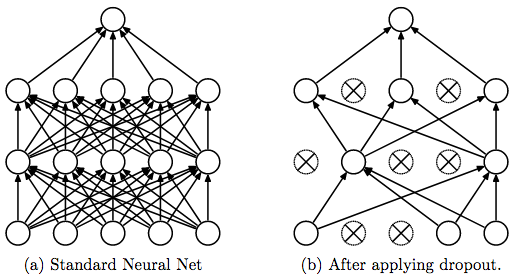
\includegraphics[width=0.7\textwidth]{figures/search_hh/mva/dropout_illustration}
        \caption{
            Illustration of dropout regularization. Figure taken from Ref.~\cite{JMLRDropout}.
            \textit{\textbf{Left}}: A standard neural network with two fully-connected layers.
            \textit{\textbf{Right}}: An example of a thinned network produced by applying dropout to the
                network on the left.
                The units with `X' have been dropped.
        }
        \label{fig:dropout_illustration}
    \end{center}
\end{figure}

\begin{figure}[!htb]
    \begin{center}
        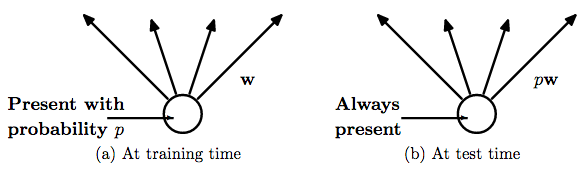
\includegraphics[width=0.7\textwidth]{figures/search_hh/mva/dropout_weight_scaling}
        \caption{
            Illustration of the dropout rate effect on the network weights. Figure taken from Ref.~\cite{JMLRDropout}.
            \textit{\textbf{Left}}: A node in a fully-connected layer at training time is present in the network with
                a probability equal to the dropout rate and is connected to the next layer with weights represented by $\bm{w}$.
            \textit{\textbf{Right}}: At test time, the node is present with 100\% probability but its weights are scaled down by the
                dropout rate, $p\bm{w}$.
        }
        \label{fig:dropout_weight_scaling}
    \end{center}
\end{figure}

\noindent
As mentioned above, the use of dropout regularization prevents nodes within the network from co-adapting
too much and forces the network to learn more robust features that are useful in conjunction with many 
different random subsets of the other nodes.
That is, dropout regularization ensures that the model is robust against the loss of any individual
``piece of evidence'' and is found to reduce the effects of overtraining, which improves the generalizability
of the trained classifier.

The neural network classifier used in the present analysis, illustrated in Figure~\ref{fig:nn_arch},
uses a single dropout layer acting on the first fully-connected node and is given a dropout rate of 50\%.

During training, the loss metric is the categorical crossentropy and the Adam optimization algorithm~\cite{AdamOptimizer} is used.\footnote{More
on categorical cross-entropy: \href{https://ml-cheatsheet.readthedocs.io/en/latest/loss_functions.html\#cross-entropy}
{https://ml-cheatsheet.readthedocs.io/en/latest/loss\_functions.html\#cross-entropy}}


%%%%%%%%%%%%%%%%%%%%%%%%%%%%%%%%%%%%%%%%%%%%%%%%%%%%%%%%%%%%%%%%%%%%%%%%%%%%%%%%%%%
%%%%%%%%%%%%%%%%%%%%%%%%%%%%%%%%%%%%%%%%%%%%%%%%%%%%%%%%%%%%%%%%%%%%%%%%%%%%%%%%%%%
%%%%%%%%%%%%%%%%%%%%%%%%%%%%%%%%%%%%%%%%%%%%%%%%%%%%%%%%%%%%%%%%%%%%%%%%%%%%%%%%%%%
%
% TRAINING AND ARCHITECTURE
%
%%%%%%%%%%%%%%%%%%%%%%%%%%%%%%%%%%%%%%%%%%%%%%%%%%%%%%%%%%%%%%%%%%%%%%%%%%%%%%%%%%%
%%%%%%%%%%%%%%%%%%%%%%%%%%%%%%%%%%%%%%%%%%%%%%%%%%%%%%%%%%%%%%%%%%%%%%%%%%%%%%%%%%%
%%%%%%%%%%%%%%%%%%%%%%%%%%%%%%%%%%%%%%%%%%%%%%%%%%%%%%%%%%%%%%%%%%%%%%%%%%%%%%%%%%%
\subsection{Definition of the Training Sample}
\label{sec:nn_train}

Prior to training a multi-variate classifier, such as the neural network described in Section~\ref{sec:nn_arch},
a well-defined set of simulated events for all labelled processed must be set aside for use in the training.
Ideally, these events are not to be used in the actual analysis, when the trained classifier is used only
for inference.
These two sets are referred to as the \textit{training set} and \textit{testing set}, respectively.

For defining our split between training and testing sets, the present analysis uses the `hold-out method' wherein
a fraction of the training events are set aside for use in evaluating classifier performance metrics
during the classifier training.
This is illustrated in Figure~\ref{fig:nn_sample_split}, where we use, out of our entire set of MC simulated
events, a percentage ($a\%$) for defining the training sample, with subsets of this set aside for evaluation
of the training performance.

\begin{figure}[!htb]
    \begin{center}
        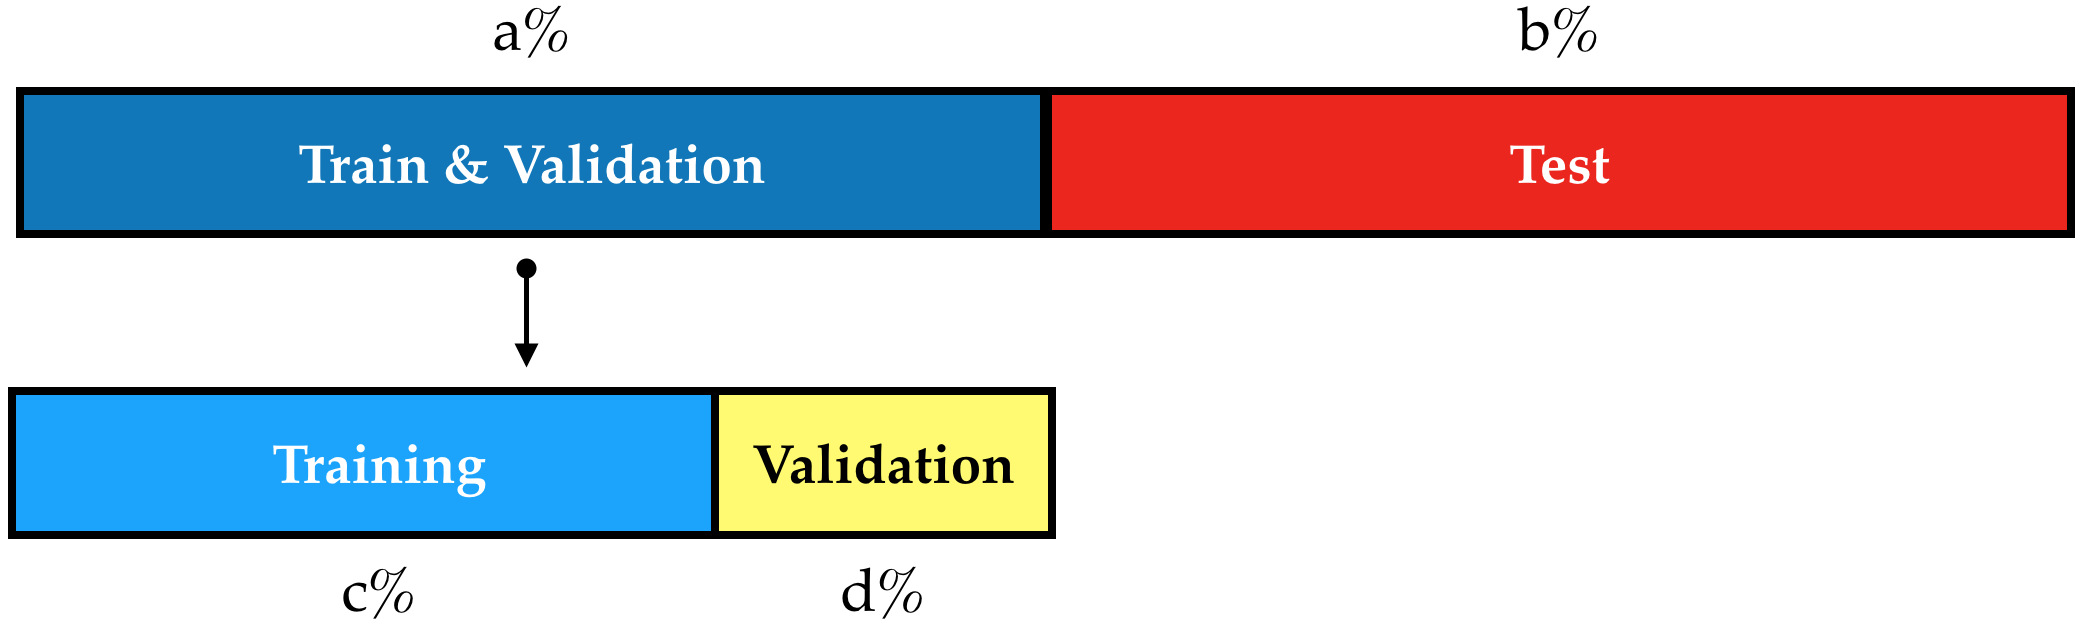
\includegraphics[width=0.7\textwidth]{figures/search_hh/mva/wwbb_nn_sample_breakdown}
        \caption{
            Illustration of the sample split used for training and testing the classifier.
            `Test' refers to the sample of events used at the analysis level (classifier inference only).
            `Training' and `Validation' events are used only during the training stage:
            Those events marked as `Training' are used for training of the classifier and those
            marked as `Validation' are used to evaluate the network performance metrics throughout
            the training process.
            $a$ is the percentage of the sample used for training and validation, $b$ the percentage used
            in the analysis, $c$ is the percentage of the Training data used for network training, and $d$ is the percentage
            of the Training data used for evaluating performance metrics.
            This gives $a\% + b\% = 100\%$ and $c\% + d\% = a\%$.
        }
        \label{fig:nn_sample_split}
    \end{center}
\end{figure}

During the training, the network is presented with inputs from MC-simulated events from each of the
four processed described above, each of which having a corresponding network output label.
The method used ensures an equal balance of processes in the training sample and revolves around
the total number of events existing in the MC sample of the signal process.
The number of events corresponding to $50\%$ of the total number of events in the signal MC sample
is set aside from each of the four samples to be used for training: $hh$, Top, $Z\rightarrow \{ee,\mu\mu\}$,
and $Z \rightarrow \tau\tau$.
The sum of all of these events corresponds to the `Training' sample in Figure~\ref{fig:nn_sample_split}.
As the neural network is trained, we want to make sure that at any given moment in the training process that the
network has a roughly equal chance of being presented with an event from any one of the four possible processes.
This ensures that no biases are learned by the network simply as a result of having an imbalanced training sample.
To avoid this, the training sample is randomly shuffled such that events in the Training sample are evenly distributed.
This breakdown and shuffling of the training events is illustrated in Figure~\ref{fig:nn_sample_shuffle}.
For the neural network trained in the present analysis, 20\% of the Training sample is set aside to make up
the Validation sample.

In addition to equally balancing the number of representative examples of each of the classes
that the neural network will be trained to identify, the MC events are not weighted during the training.
That is, the MC events are not weighted to their typical MC event weights associated with their
cross-section, reconstruction efficiencies, etc... nor are they given specific global class weights in the training.
All processes therefore have equal weight and equal sampling from the perspective of the training of the
classifier.
In the end, these parameters are additional \textit{hyperparameters} entering the training that must individually be tuned, if it is
desired to do so.
The choices made here, with respect to the process sampling and weighting, were made with the aim of designing the simplest training procedure possible.

All events used in the training procedure are required to satisfy the analysis' preselection
requirements defined in Section~\ref{sec:hh_event_selection} as well as having at least one $b$-tagged
jet, as detailed in Table~\ref{tab:train_selection}.
This is a rather loose selection --- looser than the one that will eventually be applied in the definition
of the analysis' SRs, CRs, and VRs --- but allows for larger numbers of events to be used in the training
process.

\begin{figure}[!htb]
    \begin{center}
        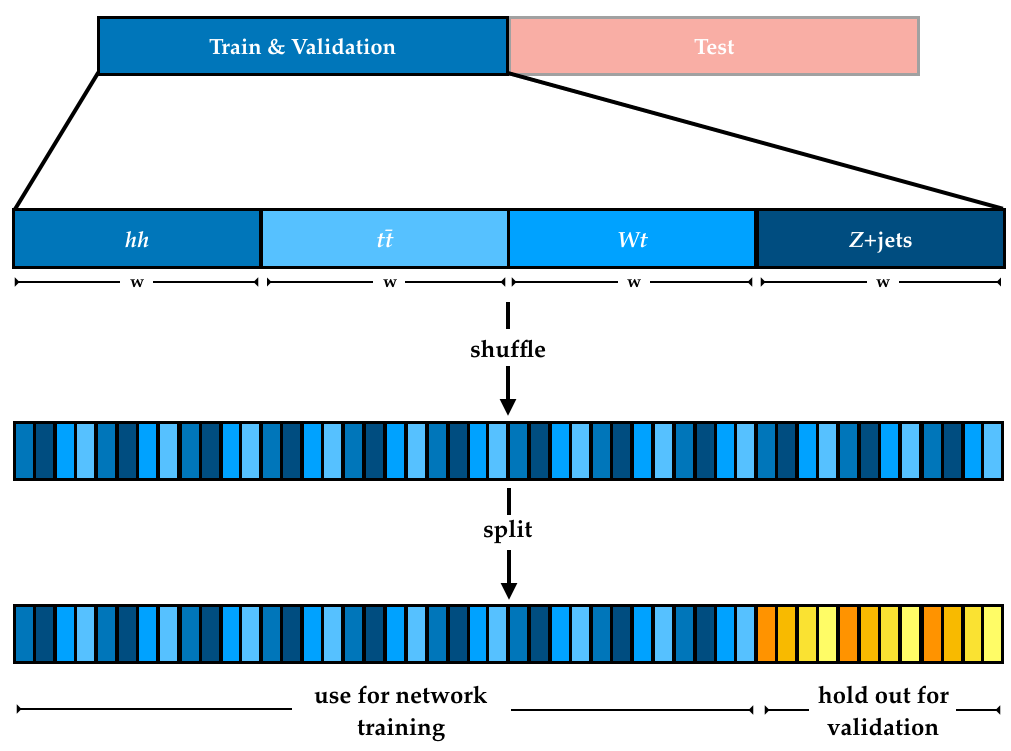
\includegraphics[width=0.8\textwidth]{figures/search_hh/mva/wwbb_nn_sample_split_detail}
        \caption{
            Detailed illustration of how the allocated training data is split into separate training
            and validation data samples.
            The sample size, or width $\bm{w}$, is defined by the signal MC sample: $\bm{w}$ is defined
            to be half of the events available in the signal MC.
            This width defines the sample sizes of the remaining three processes for which the neural network
            classifier provides an output label.
            Before the training process begins, these samples are randomly shuffled such that each process is distributed
            evenly throughout the entire set of events set aside for training.
            The validation sample is defined by holding out 20\% of the shuffled data.
            Labels and scales in the figure are illustrative only.
        }
        \label{fig:nn_sample_shuffle}
    \end{center}
\end{figure}

\begin{table}[!htb]
    \begin{center}
        \caption{
            Selection applied to events used in the neural network classifier training.
            In addition to this selection, the events must pass the standard preselection
            defined in Section~\ref{sec:hh_event_selection}.
        }
        \label{tab:train_selection}
        \begin{tabular}{l|c}
        \hline
        \hline
            \textbf{Observable} & \textbf{Selection} \\
            \hline
            Analysis preselection & Applied \\
            $b$-tagged jet multiplicity & $\ge 1$ \\
        \hline
        \hline
        \end{tabular}
    \end{center}
\end{table}

%%%%%%%%%%%%%%%%%%%%%%%%%%%%%%%%%%%%%%%%%%%%%%%%%%%%%%%%%%%%%%%%%%%%%%%%%%%%%%%%%%%
%%%%%%%%%%%%%%%%%%%%%%%%%%%%%%%%%%%%%%%%%%%%%%%%%%%%%%%%%%%%%%%%%%%%%%%%%%%%%%%%%%%
%%%%%%%%%%%%%%%%%%%%%%%%%%%%%%%%%%%%%%%%%%%%%%%%%%%%%%%%%%%%%%%%%%%%%%%%%%%%%%%%%%%
%
% PREPROCESSING
%
%%%%%%%%%%%%%%%%%%%%%%%%%%%%%%%%%%%%%%%%%%%%%%%%%%%%%%%%%%%%%%%%%%%%%%%%%%%%%%%%%%%
%%%%%%%%%%%%%%%%%%%%%%%%%%%%%%%%%%%%%%%%%%%%%%%%%%%%%%%%%%%%%%%%%%%%%%%%%%%%%%%%%%%
%%%%%%%%%%%%%%%%%%%%%%%%%%%%%%%%%%%%%%%%%%%%%%%%%%%%%%%%%%%%%%%%%%%%%%%%%%%%%%%%%%%

\subsection{Input Features and their Preprocessing}
\label{sec:nn_preprocessing}

The thirty five inputs to the neural network are detailed in Table~\ref{tab:nn_inputs}.
They are composed of low level features of the visible final state objects, such
as the lepton and jet momenta, as well as observables sensitive to the Higgs hemisphere
topology characterising the dilepton $hh \rightarrow \bbww$ signal and described in Section~\ref{sec:hh_pheno}.

As discussed in Section~\ref{sec:nn_train} and indicated in Table~\ref{tab:train_selection}, the neural network
classifier is trained on events with the minimal requirement that they pass the analysis preselection requirements
and that there be at least one $b$-tagged jet in the event.
One can see by comparing the training event selection in Table~\ref{tab:train_selection} and the network
inputs in Table~\ref{tab:nn_inputs}, that there will be cases where several of the input features
will be ill-defined.
Specifically, there will be cases wherein a training event has only a single $b$-tagged jet in which
case the observables listed in Table~\ref{tab:nn_inputs} that require at least two $b$-tagged jets
are not defined.
What is done in these cases is to fix the two $b$-tagged jet observables in Table~\ref{tab:nn_inputs}
for these one $b$-tagged jet events to the \textit{mean} of the corresponding observable as seen in
those events that have at least two $b$-tagged jets.
The mean for each observable is defined using as sample of events all those events that make
up the training sample, inclusive of all four of the trained-against processes.
That is, distributions of all observables are constructed for each of four processes ($hh$, Top, $Z \rightarrow \{ee,\mu\mu\}$, $Z \rightarrow \tau\tau$)
for those events with at least two $b$-tagged jets.
For each observable, the four process-specific distributions are summed together to produce the final
distribution from which the mean value is extracted.
During the network training, these mean values are used for the observables requiring
at least two $b$-tagged jets to be defined in those events only having a single $b$-tagged jet.
This procedure, illustrated in Figure~\ref{fig:nn_feature_means}, is done only during the training phase of the classifier.

A second stage of input feature pre-processing is applied to all features provided to the classifier,
done at both the training and in the testing stage of the analysis.
This stage is a standardization step and involves, for each event, the shifting of each input feature by its mean value and scaling
its value by its pre-shifted variance,
\begin{align*}
    x^{\prime} = \frac{x - \langle x \rangle}{\sigma_x}.
\end{align*}
This type of standardization is fairly standard practice, and is done so that all inputs provided
to the neural network are on a similar range --- centered at zero and with common spread --- thereby
making it easier for the classifier to learn the relationships (i.e. correlations) between the inputs,
as opposed to their absolute scales.
These standardization schemes additionally aid in numerically stabilizing the neural network's gradient-descent-based
optimization procedures employed during the training phase.
The standardization described above and used in the present analysis is illustrated in Figure~\ref{fig:nn_feature_standard}.


\begin{table}[!htb]
    \begin{center}
    \begin{footnotesize}
    \caption{
        Description of the variables used as inputs to the DNN classifier.
    }
    \label{tab:nn_inputs}
    \begin{tabularx}{\textwidth}{l |p{14.5cm}l}
    \toprule
    \hline
    ($p_{T}$, $\eta$, $\phi$) & $p_{T}$, $\eta$, and $\phi$ of the leptons, leading two signal jets, and leading two $b$-tagged jets \\
    Dilepton flavour & Whether the event is composed of two electrons, two muons, or one of each \\
    $\Delta R_{\ell\ell}$, $|\Delta \phi_{\ell\ell}|$   & $\Delta R$ and magnitude of the $\Delta \phi$ between the two leptons \\
    $m_{\ell\ell}$, $p_{T}^{\ell\ell}$  & Invariant mass and the transverse momentum of the dilepton system \\
    $\met$, $\met$-$\phi$ & Magnitude of the missing transverse momentum vector and its $\phi$ component \\
    $|\Delta \phi (\ptmiss, \ptvec{\ell}{\ell})|$ & Magnitude of the $\Delta \phi$ between the \ptmiss and the transverse momentum of the dilepton system \\
    $|\ptmiss + \ptvec{\ell}{\ell}|$ & Magnitude of the vector sum of the \ptmiss and the transverse momentum of the dilepton system \\
    Jet multiplicities & Numbers of $b$-tagged and non-$b$-tagged jets \\
    $|\Delta \phi_{bb}|$ & Magnitude of the $\Delta \phi$ between the leading two $b$-tagged jets \\ [0.08cm]
    $\mtbb$ & \mttwo using the leading two $b$-tagged jets as the visible inputs and \ptmiss as invisible input\\ [0.1cm]
    $\httwo$ & Numerator appearing in Equation~\ref{eq:ht2ratio_def}, \htnum \\
    $\htratio$ & As defined in Equation~\ref{eq:ht2ratio_def} \\
    \hline
    \bottomrule
    \end{tabularx}
    \end{footnotesize}
    \end{center}
\end{table}

\begin{figure}[!htb]
    \begin{center}
        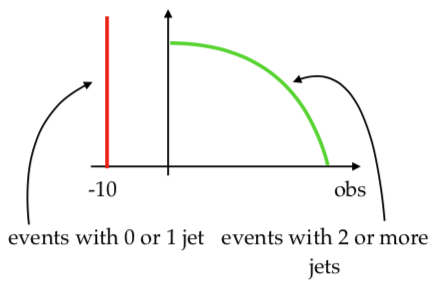
\includegraphics[width=0.45\textwidth]{figures/search_hh/mva/nn_feature_illdefined}
        \raisebox{0.5cm}{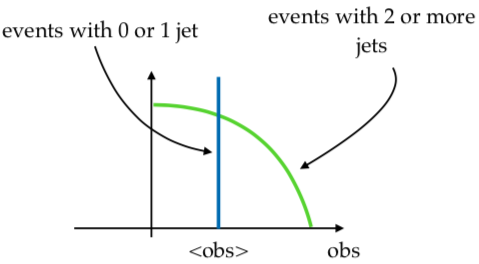
\includegraphics[width=0.54\textwidth]{figures/search_hh/mva/nn_feature_okdefined}}
        \caption{
            Illustration of setting events with ill-defined observables to the mean of those observables
            as measured in events in which the observables are properly defined.
            \textit{\textbf{Left}}: A counter-example in which ill-defined events' observables are set to a fixed default
                value outside of the physical range (a common practice).
                This would bias the mean of the properly defined events to the left.
            \textit{\textbf{Right}}: Setting the ill-defined events' observables to the mean of the observable
                as seen in events where the observable is properly defined.
                Doing this does not affect the overall mean of the observable in events where the
                observable is well-defined, nor does it lead to a discontinuity in the distributions of observables
                being provided to the classifier during its training.
        }
        \label{fig:nn_feature_means}
    \end{center}
\end{figure}

\begin{figure}[!htb]
    \begin{center}
        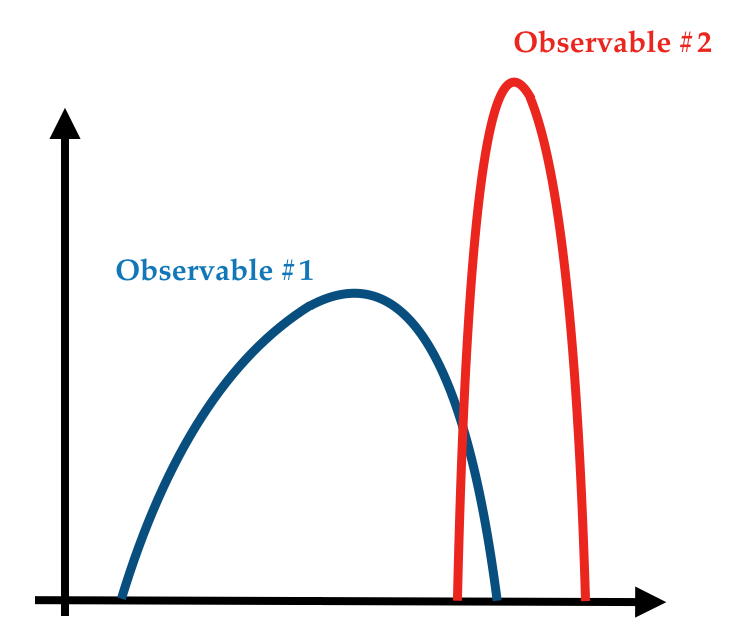
\includegraphics[width=0.38\textwidth]{figures/search_hh/mva/feature_standard_1}
        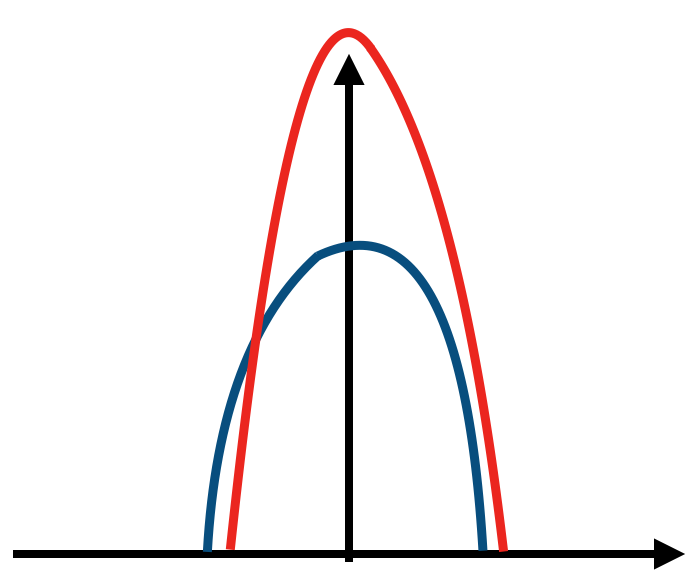
\includegraphics[width=0.38\textwidth]{figures/search_hh/mva/feature_standard_2}
        \caption{
            Illustration of the input feature standardization that occurs for all input features,
            for all events, prior to the features being fed into the neural network classifier
            (for both training and testing).
            \textit{\textbf{Left}}: Two different observables (overlaid for comparison) that have quite
            different shapes. Observable \#1 has a larger variance and is shifted to the left with
            respect to Observable \#2, which is a quite localized observable.
            \textit{\textbf{Right}}: After standardization, both observables have roughly the same
            mean (zero) and their widths have been scaled such that they are similar.
        }
        \label{fig:nn_feature_standard}
    \end{center}
\end{figure}

Note that it is this standardization procedure which motivates the method that
is used for augmenting the two $b$-tagged jet observables in the one $b$-tagged jet events.
By setting the ill-defined observables in the on $b$-tagged jet events to the mean of the observables
as defined in the two $b$-tagged jet events, we theoretically prevent the neural network from learning
from that specific observable on such events since after standardization they will be shifted towards zero
and any spurious correlation will be minimized.
In practice, however, it has been found that the specific choice of the scheme used for augmenting the two $b$-tagged jet observables
in one $b$-tagged jet events has little meaningful impact on the performance of the classifier.
The one described above has been used as it is the simplest, practically speaking.

The pre-processing steps, happening at each event and in order, are as follows:
\begin{enumerate}
    \item Augment two $b$-tagged jet observables for one $b$-tagged jet events (if applicable)
    \item Perform input feature standardization
    \item Feed inputs to network (either for training or for use in the analysis)
\end{enumerate}

%%%%%%%%%%%%%%%%%%%%%%%%%%%%%%%%%%%%%%%%%%%%%%%%%%%%%%%%%%%%%%%%%%%%%%%%%%%%%%%%%%%
%%%%%%%%%%%%%%%%%%%%%%%%%%%%%%%%%%%%%%%%%%%%%%%%%%%%%%%%%%%%%%%%%%%%%%%%%%%%%%%%%%%
%%%%%%%%%%%%%%%%%%%%%%%%%%%%%%%%%%%%%%%%%%%%%%%%%%%%%%%%%%%%%%%%%%%%%%%%%%%%%%%%%%%
%
% NN  TRAINING
%
%%%%%%%%%%%%%%%%%%%%%%%%%%%%%%%%%%%%%%%%%%%%%%%%%%%%%%%%%%%%%%%%%%%%%%%%%%%%%%%%%%%
%%%%%%%%%%%%%%%%%%%%%%%%%%%%%%%%%%%%%%%%%%%%%%%%%%%%%%%%%%%%%%%%%%%%%%%%%%%%%%%%%%%
%%%%%%%%%%%%%%%%%%%%%%%%%%%%%%%%%%%%%%%%%%%%%%%%%%%%%%%%%%%%%%%%%%%%%%%%%%%%%%%%%%%

\subsection{Training Procedure}
\label{sec:nn_train_procedure}

For illustration purposes, Figure~\ref{fig:nn_batches} illustrates the process of training
a neural network with many batches of events, the sum total of which comprise the entirety
of the events set aside for training.
An epoch refers to the point at which every single event in the training sample has been fed into
the network.
The neural network classifier described in Section~\ref{sec:nn_arch} is trained using the 
sample of events described in Section~\ref{sec:nn_train} using a batch size of 2,000 events,
with a maximum number of training epochs set to a large number ($\mathcal{O}(100)$).

Neural network classifiers typically train for many epochs, meaning that every event in the training
sample is used multiple times in the training procedure.
The training procedure used in the present analysis relies on an `early-stopping' metric that is imposed during the training phase such that, if the network's learning
begins to plateau, it will stop the training whether or not the maximum number of epochs has been
reached.
The metric used to determine whether the early-stopping criteria has been met is the neural network
loss value as evaluated on the held-out validation sample of events.
The aim of the network, during the training phase, is to minimize the loss.
Therefore, once the metric used for defining the early-stopping criteria hits a (minimum) plateau
it will stop after a configurable number of epochs in which no new minimum is found.
This configurable number, referred to as the `patience', is set to 20 for the classifier used in the present analysis.
%leading to a typical training phase lasting for 80 to 110 epochs.
Figure~\ref{fig:nn_epoch_overtrain} shows several training performance metrics evaluated on both the
training and held-out validation data, from which it can be seen that setting the patience parameter to 20
allows the network to maximize its learning before effects of overtraining begin to set in.

\begin{figure}[!htb]
    \begin{center}
        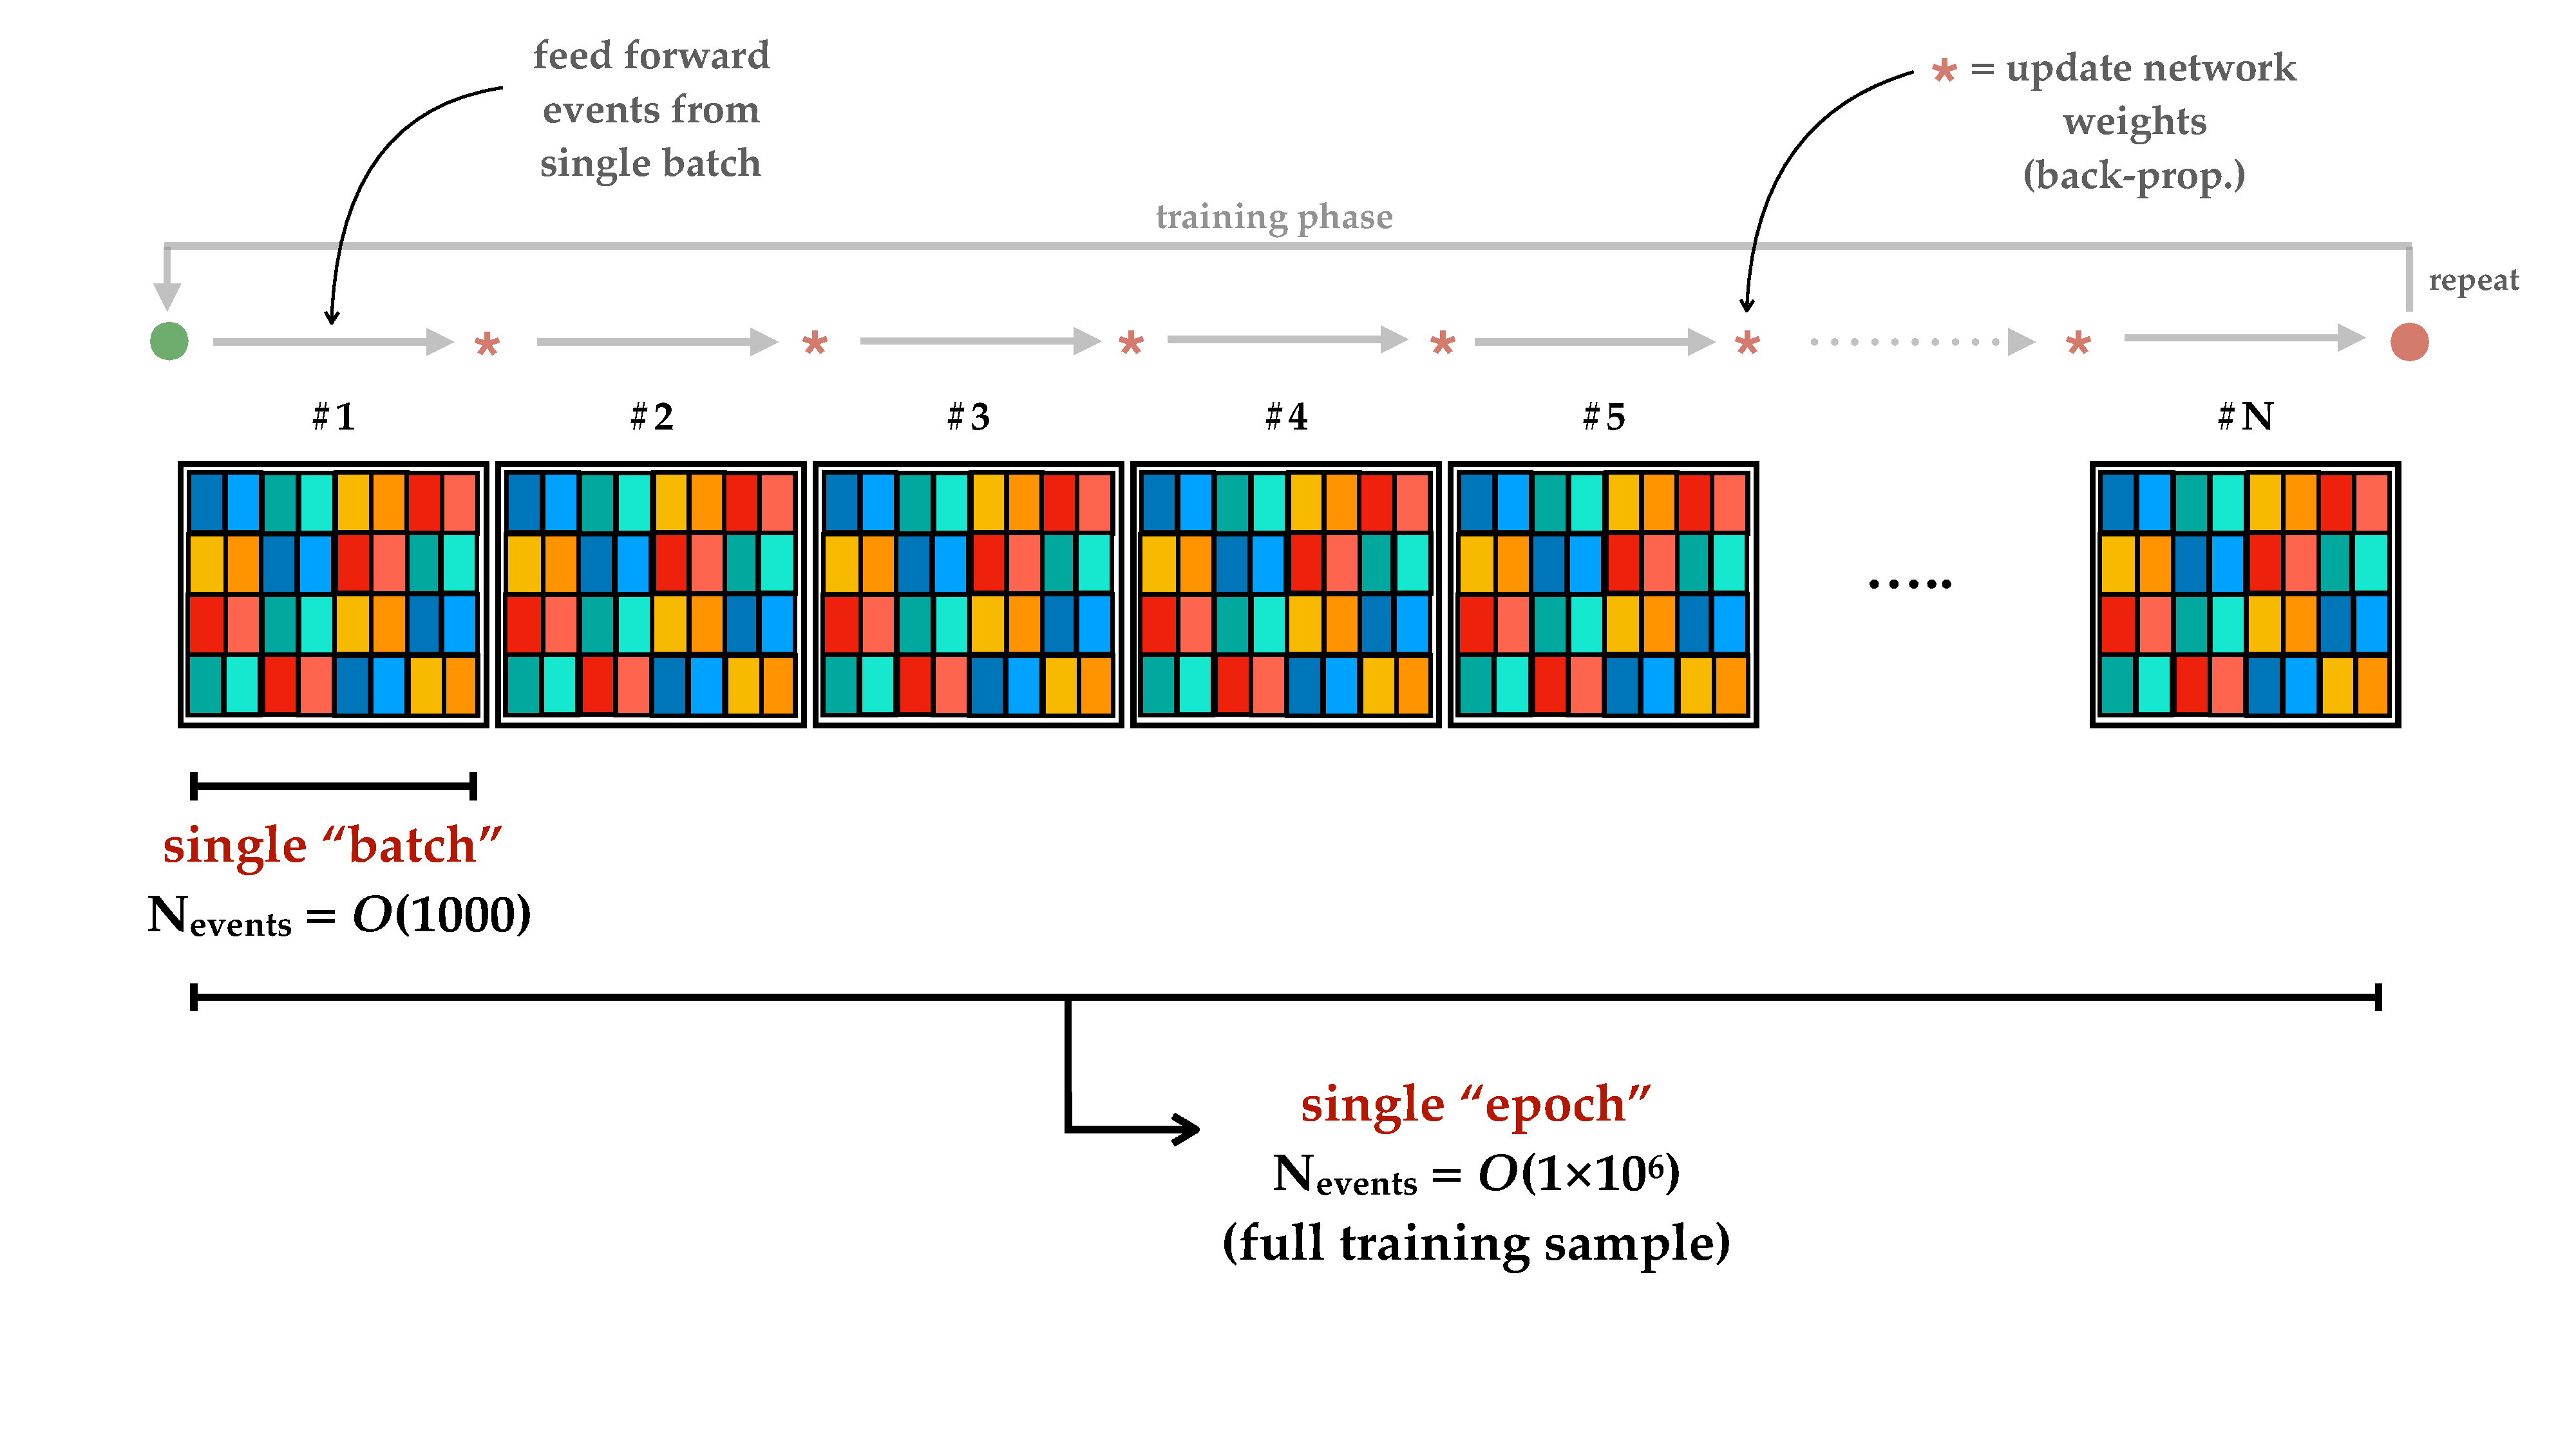
\includegraphics[width=1.0\textwidth]{figures/search_hh/mva/nn_batchesPDF}
        \caption{
            A neural network training sample is broken into many sub-samples referred to as `batches'.
            In the training phase of the neural network, the network parameters (weights and biases)
            are only updated after each batch is fed into the network.
            A training `epoch' refers to the point in the training at which all of the events
            in the entire training sample have been fed forward through the network for training purposes.
            The size of each batch (i.e. the number of events that are in a batch), as well as the number
            epochs to train for, are configurable parameters that must be optimized.
            See Ref.~\cite{GoodFellowBook} for more information.
        }
        \label{fig:nn_batches}
    \end{center}
\end{figure}

\begin{figure}[!htb]
    \begin{center}
        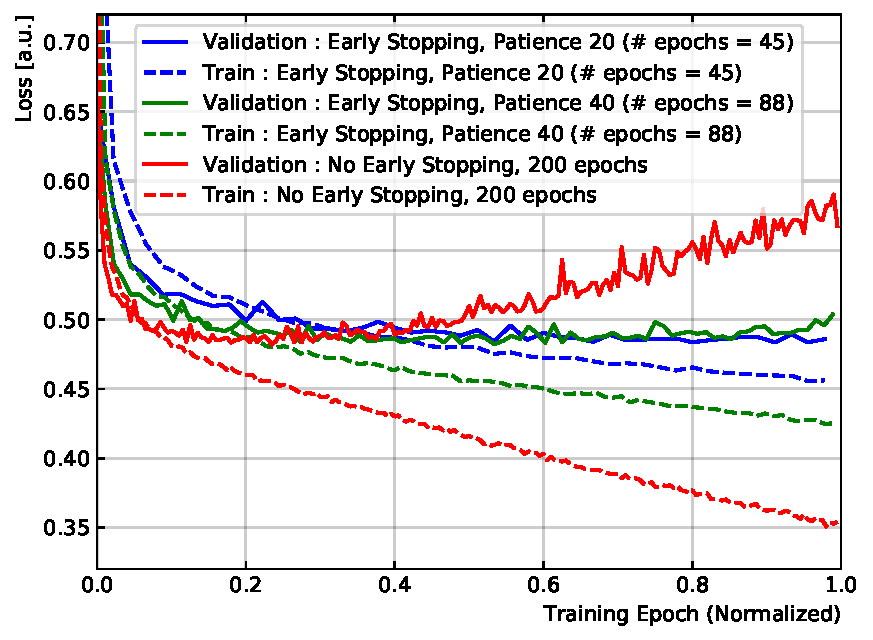
\includegraphics[width=0.48\textwidth]{figures/search_hh/mva/overtrain_check_loss}
        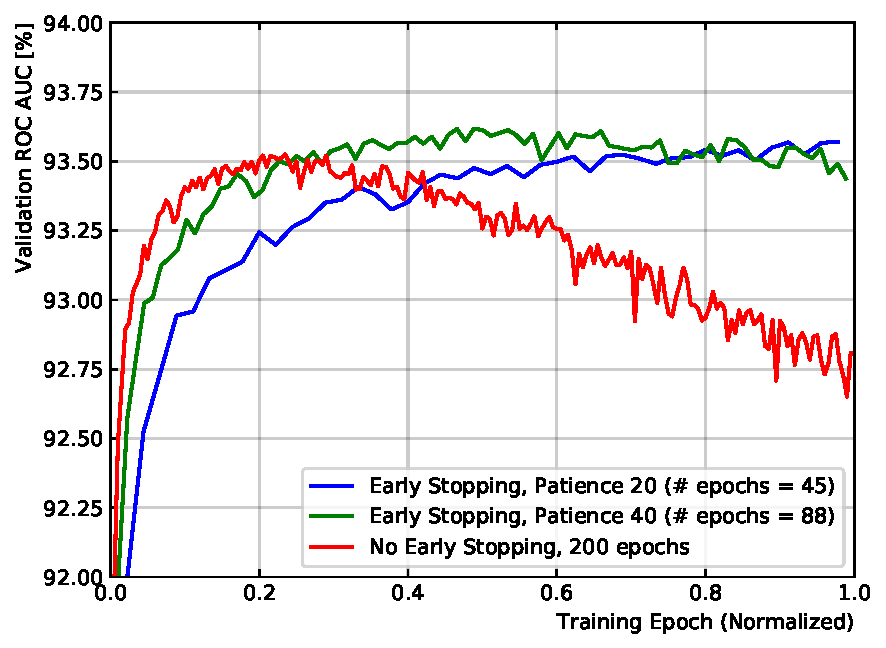
\includegraphics[width=0.48\textwidth]{figures/search_hh/mva/overtrain_check_roc_auc}
        \caption{
            \textit{\textbf{Left}}: The neural network loss as a function of the number of training epochs.
                The solid lines report the loss evaluated on the held-out validation sample of events,
                while the dashed lines report that evaluated using the sample of events used for training.
                The larger discrepancy observed between the validation and training loss observed in the
                cases where the training is allowed to proceed for a larger number of epochs indicate
                larger amounts of overtraining.
            \textit{\textbf{Right}}: Receiver operating characteristic area-under-the-curve (ROC AUC), evaluated using
                the held-out validation sample of events, as a function of the number of training epochs.
                Larger values of ROC AUC indicate better network classification performance.
                The drop in ROC AUC observed in the green and red curves are a result of increased levels
                of overtraining, resulting in the classifier being unable to generalize to data other than
                that used for training.
        }
        \label{fig:nn_epoch_overtrain}
    \end{center}
\end{figure}

%%%%%%%%%%%%%%%%%%%%%%%%%%%%%%%%%%%%%%%%%%%%%%%%%%%%%%%%%%%%%%%%%%%%%%%%%%%%%%%%%%%
%%%%%%%%%%%%%%%%%%%%%%%%%%%%%%%%%%%%%%%%%%%%%%%%%%%%%%%%%%%%%%%%%%%%%%%%%%%%%%%%%%%
%%%%%%%%%%%%%%%%%%%%%%%%%%%%%%%%%%%%%%%%%%%%%%%%%%%%%%%%%%%%%%%%%%%%%%%%%%%%%%%%%%%
%
% NN DISCRIMINANTS
%
%%%%%%%%%%%%%%%%%%%%%%%%%%%%%%%%%%%%%%%%%%%%%%%%%%%%%%%%%%%%%%%%%%%%%%%%%%%%%%%%%%%
%%%%%%%%%%%%%%%%%%%%%%%%%%%%%%%%%%%%%%%%%%%%%%%%%%%%%%%%%%%%%%%%%%%%%%%%%%%%%%%%%%%
%%%%%%%%%%%%%%%%%%%%%%%%%%%%%%%%%%%%%%%%%%%%%%%%%%%%%%%%%%%%%%%%%%%%%%%%%%%%%%%%%%%

\subsection{Classifier Discriminants}
\label{sec:nn_discriminants}

The multi-output classifier described in Section~\ref{sec:nn_arch} provides four outputs for each event
once provided an input feature vector.
In our case, the four outputs are taken to loosely represent the probabilities, or strengths, that the
set of inputs correspond to one of the four labels for which the classifier has been trained to distinguish.
We refer to these outputs, then, as \phh, \ptop, \pzsf, and \pztt
for the $hh$, Top, $Z\rightarrow \{ee,\mu\mu\}$, and $Z\rightarrow \tau\tau$ process labels, respectively.
Representative distributions for each of the $p_i$, for the corresponding signal and background processes,
are shown in Figure~\ref{fig:nn_disc_p}.

From the set of $p_i$, we build a set of four composite discriminants, each of which combines information
contain within them all.
These discriminants are log-ratio discriminants of the output scores, defined in Equation~\ref{eq:nn_disc_def}.
Representative distributions for each of the composite discriminants are shown in Figure~\ref{fig:nn_disc_d}.
The discriminant \dhh is the primary observable around which the SRs, CRs, and VRs are defined
in the present analysis.

\begin{align}
    d_Q = \ln \left( \frac{p_Q}{p_X + p_Y + p_Z} \right)
    \label{eq:nn_disc_def}
\end{align}

\begin{figure}[!htb]
    \begin{center}
        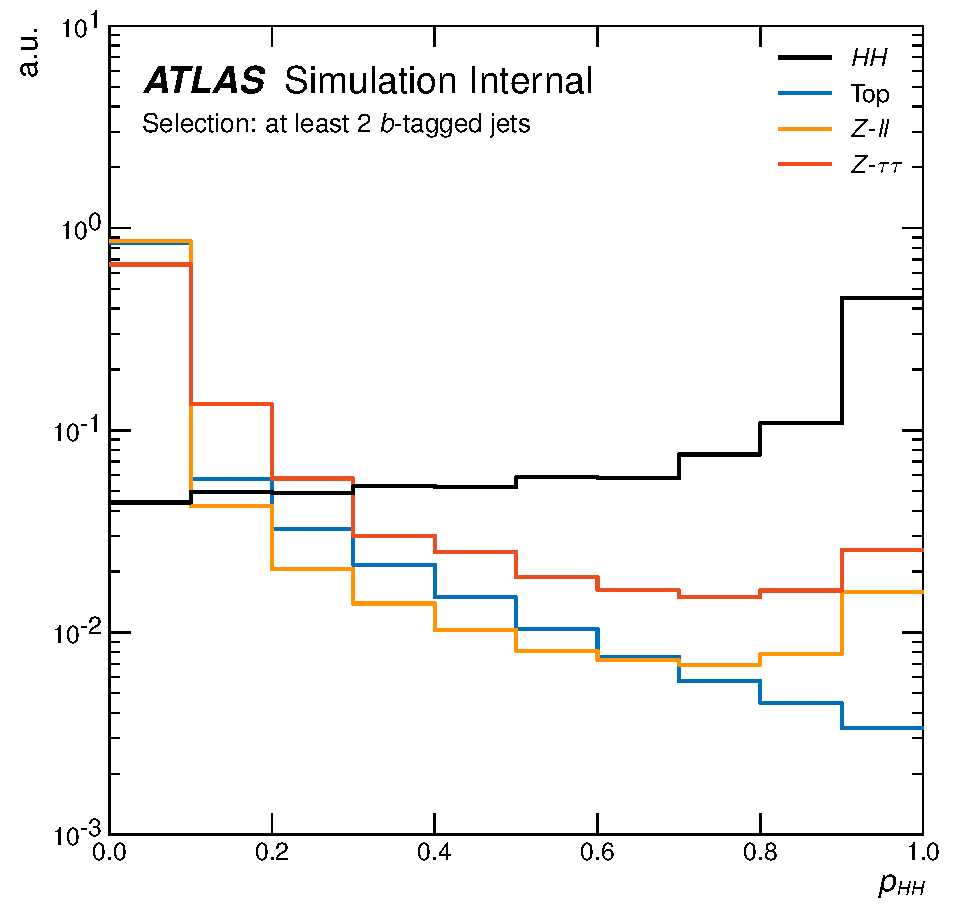
\includegraphics[width=0.48\textwidth]{figures/search_hh/nn_disc/pi_plot_NN_p_hh}
        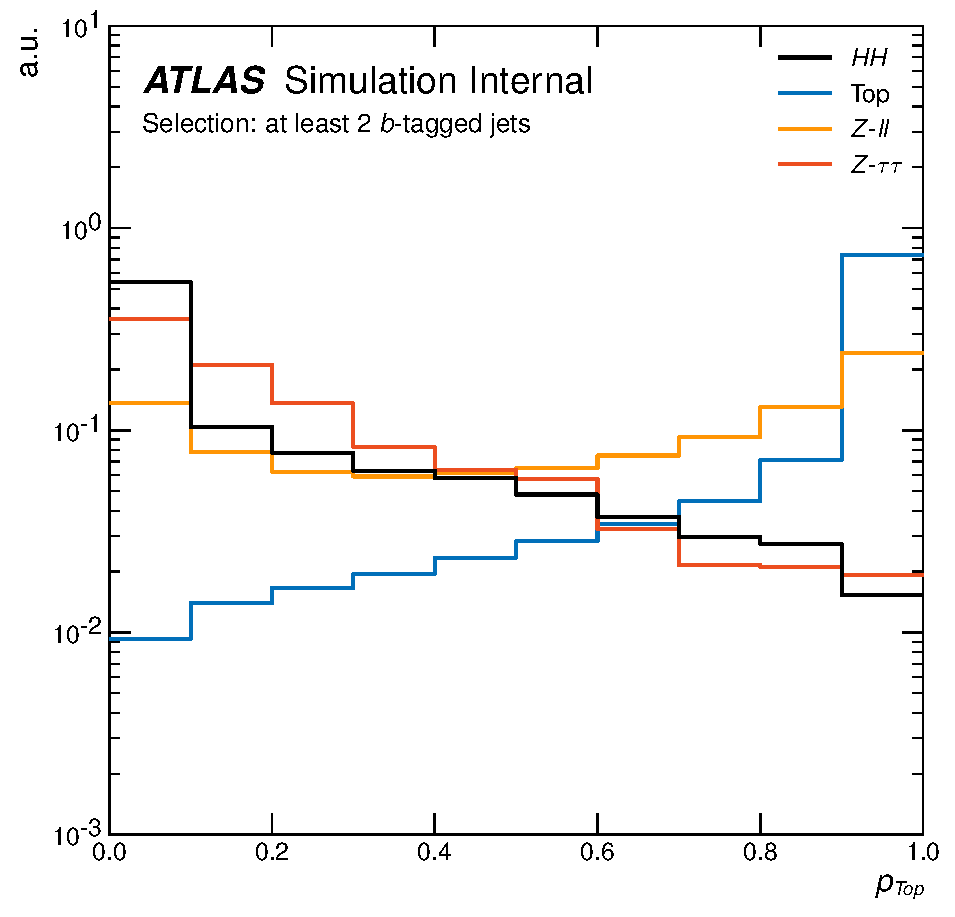
\includegraphics[width=0.48\textwidth]{figures/search_hh/nn_disc/pi_plot_NN_p_top}
        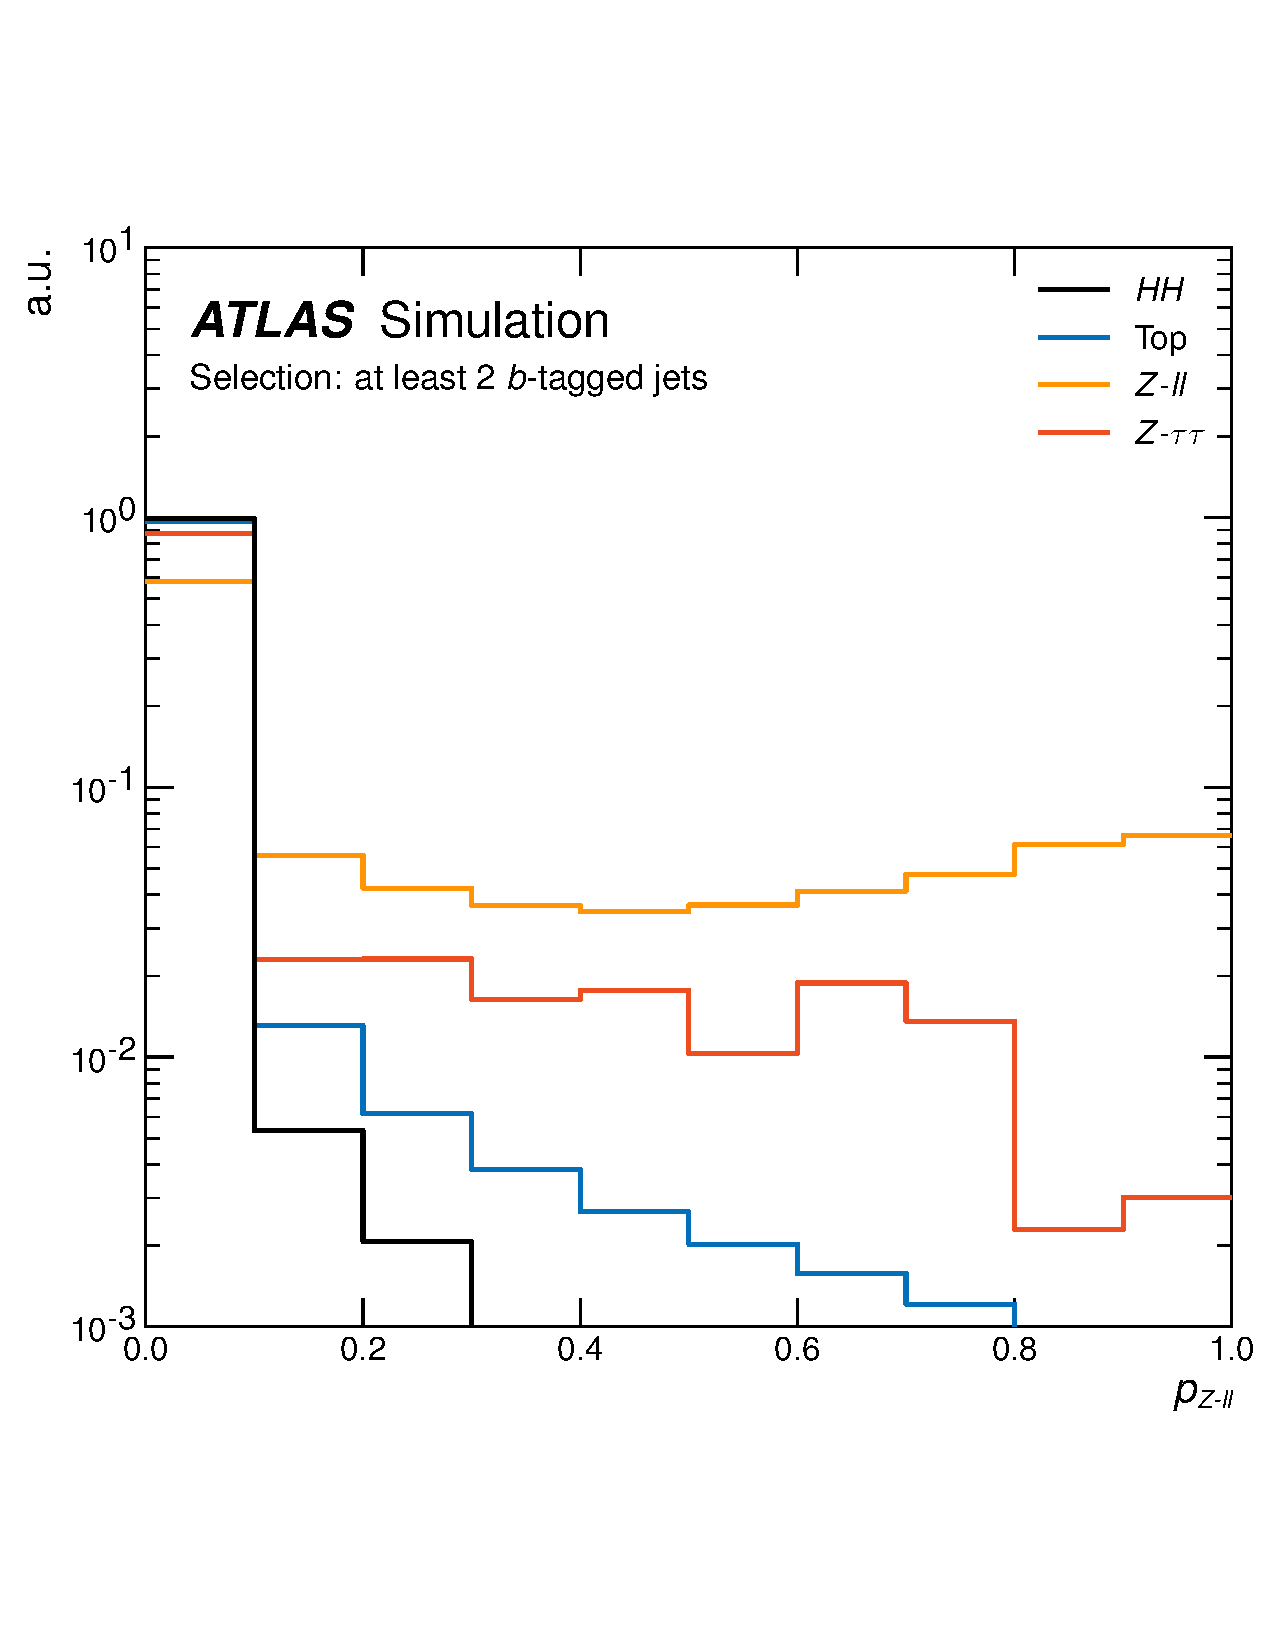
\includegraphics[width=0.48\textwidth]{figures/search_hh/nn_disc/pi_plot_NN_p_zsf}
        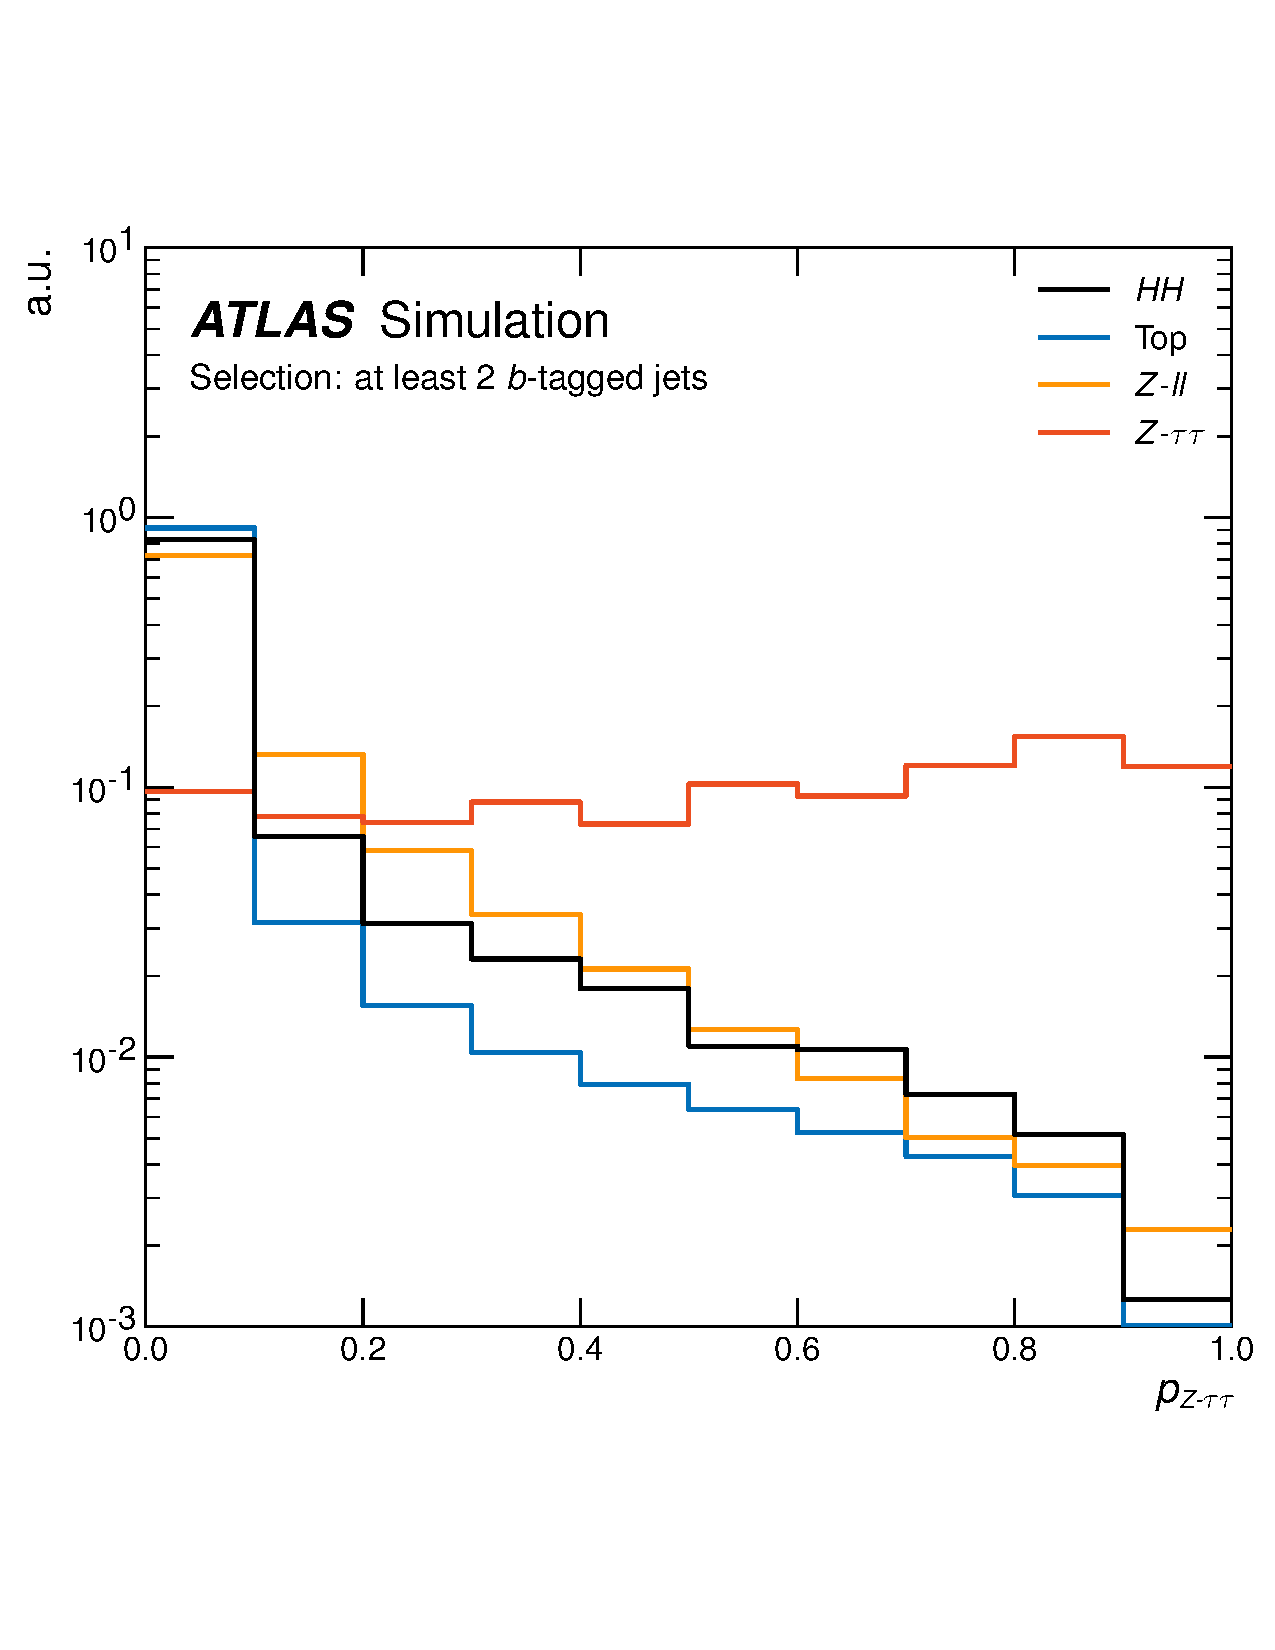
\includegraphics[width=0.48\textwidth]{figures/search_hh/nn_disc/pi_plot_NN_p_ztt}
        \caption{
            Normalized distributions of the four network outputs,
            shown for the dilepton
            $hh \rightarrow \bbww$ signal (black), Top (blue), $Z \rightarrow \{ee,\mu\mu\}$ (yellow),
            and $Z\rightarrow \tau\tau$ (orange) processes.
            From the top left and moving clock-wise: \phh, \ptop, \pztt, and \pzsf.
        }
        \label{fig:nn_disc_p}
    \end{center}
\end{figure}

\begin{figure}[!htb]
    \begin{center}
        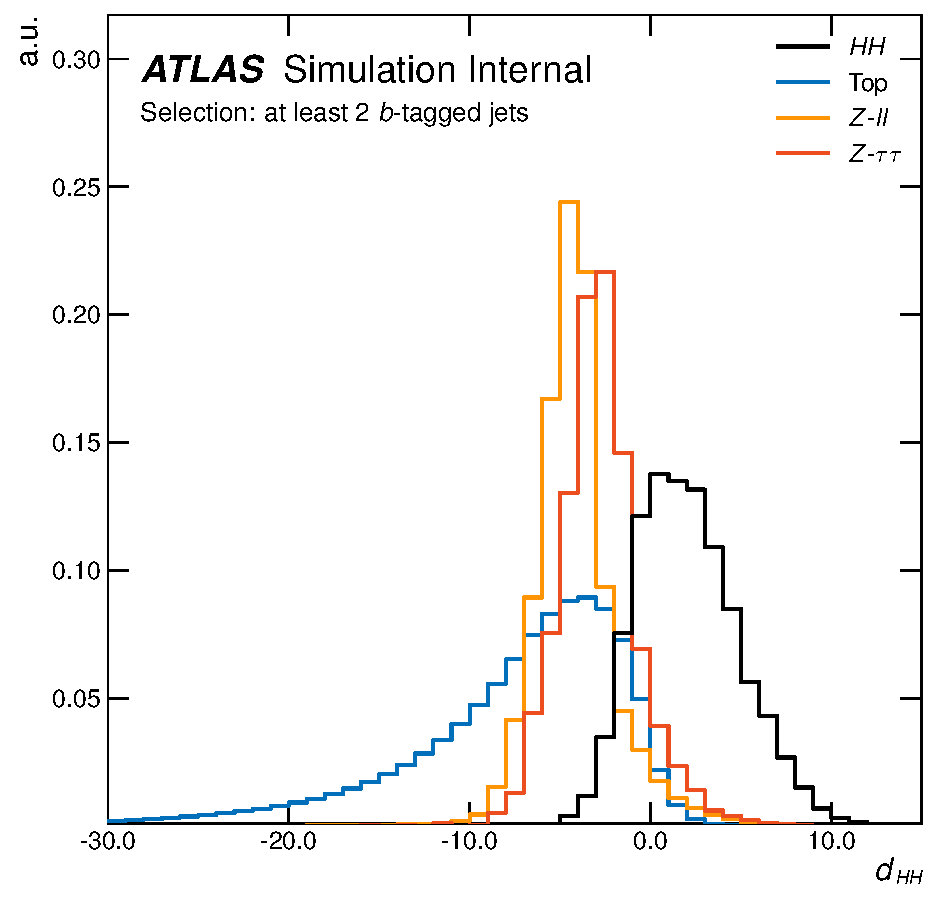
\includegraphics[width=0.48\textwidth]{figures/search_hh/nn_disc/pi_plot_NN_d_hh}
        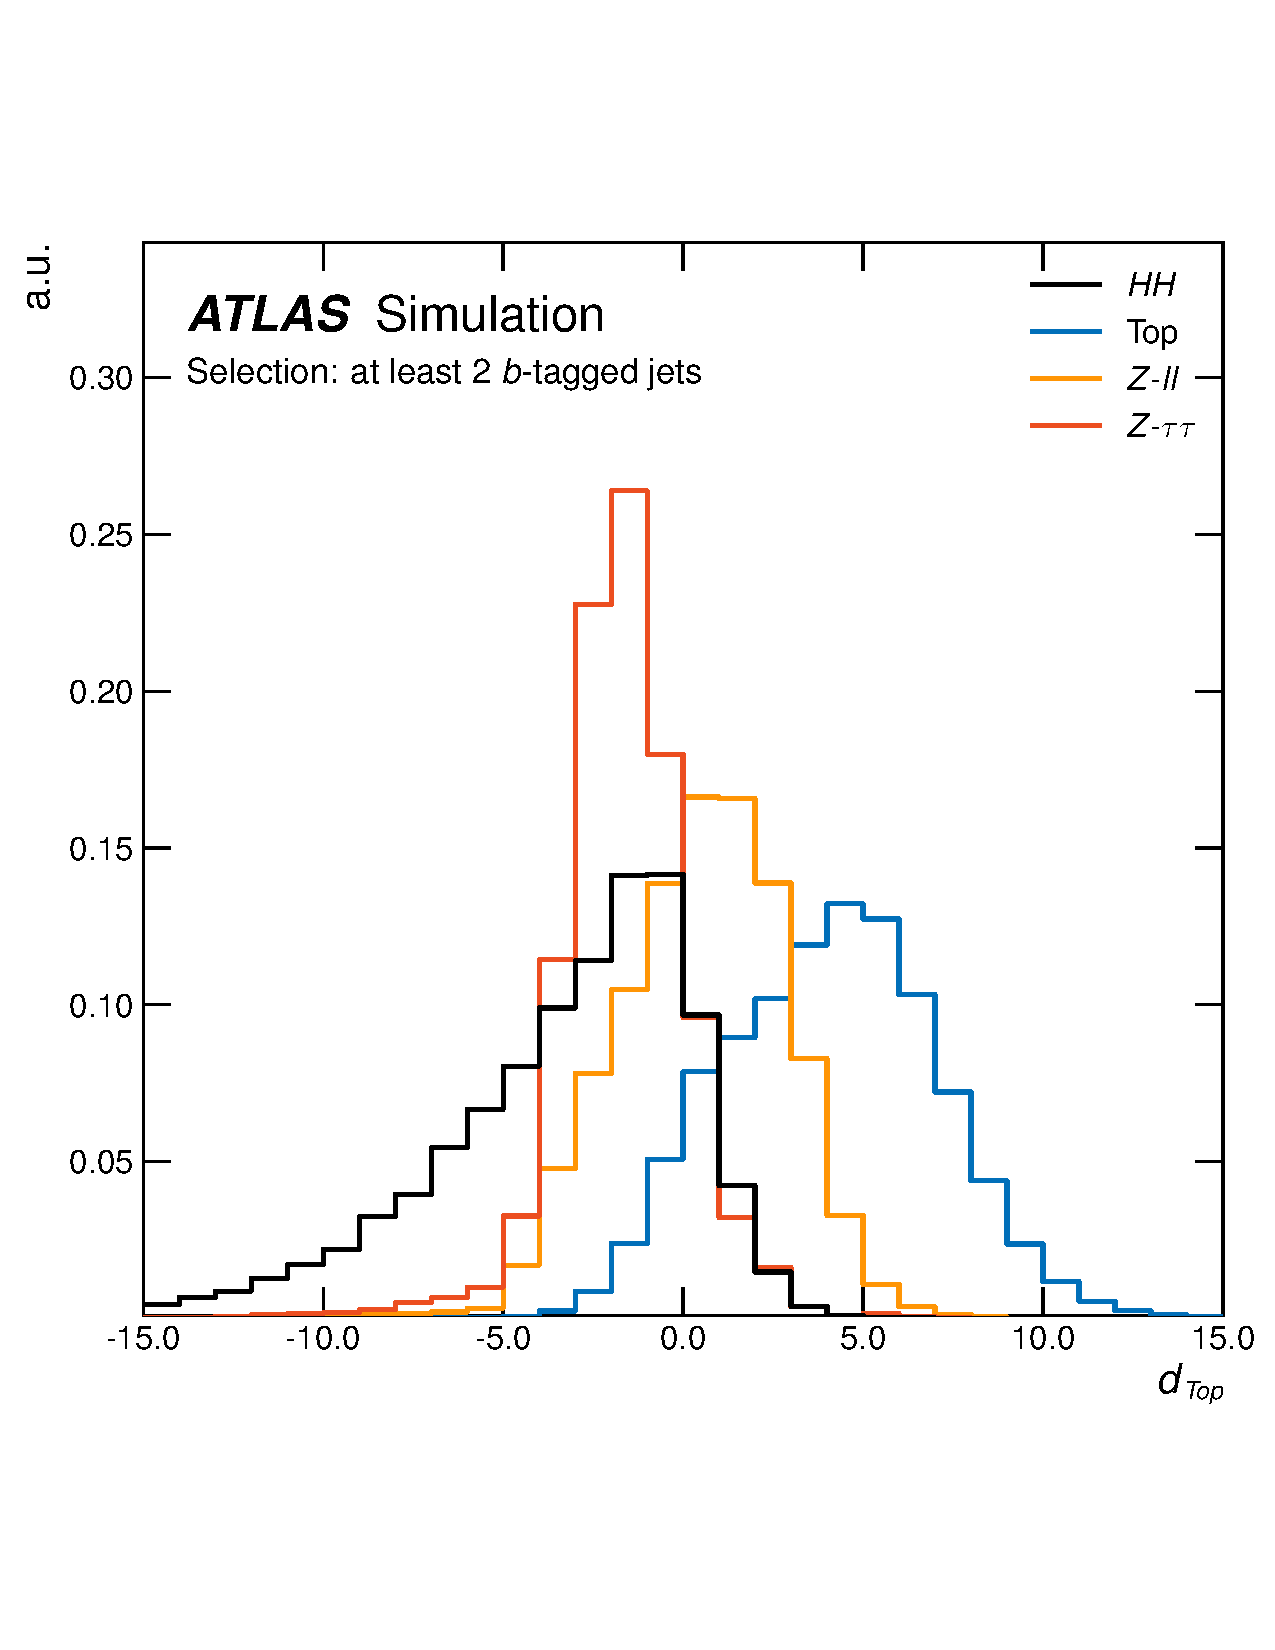
\includegraphics[width=0.48\textwidth]{figures/search_hh/nn_disc/pi_plot_NN_d_top}
        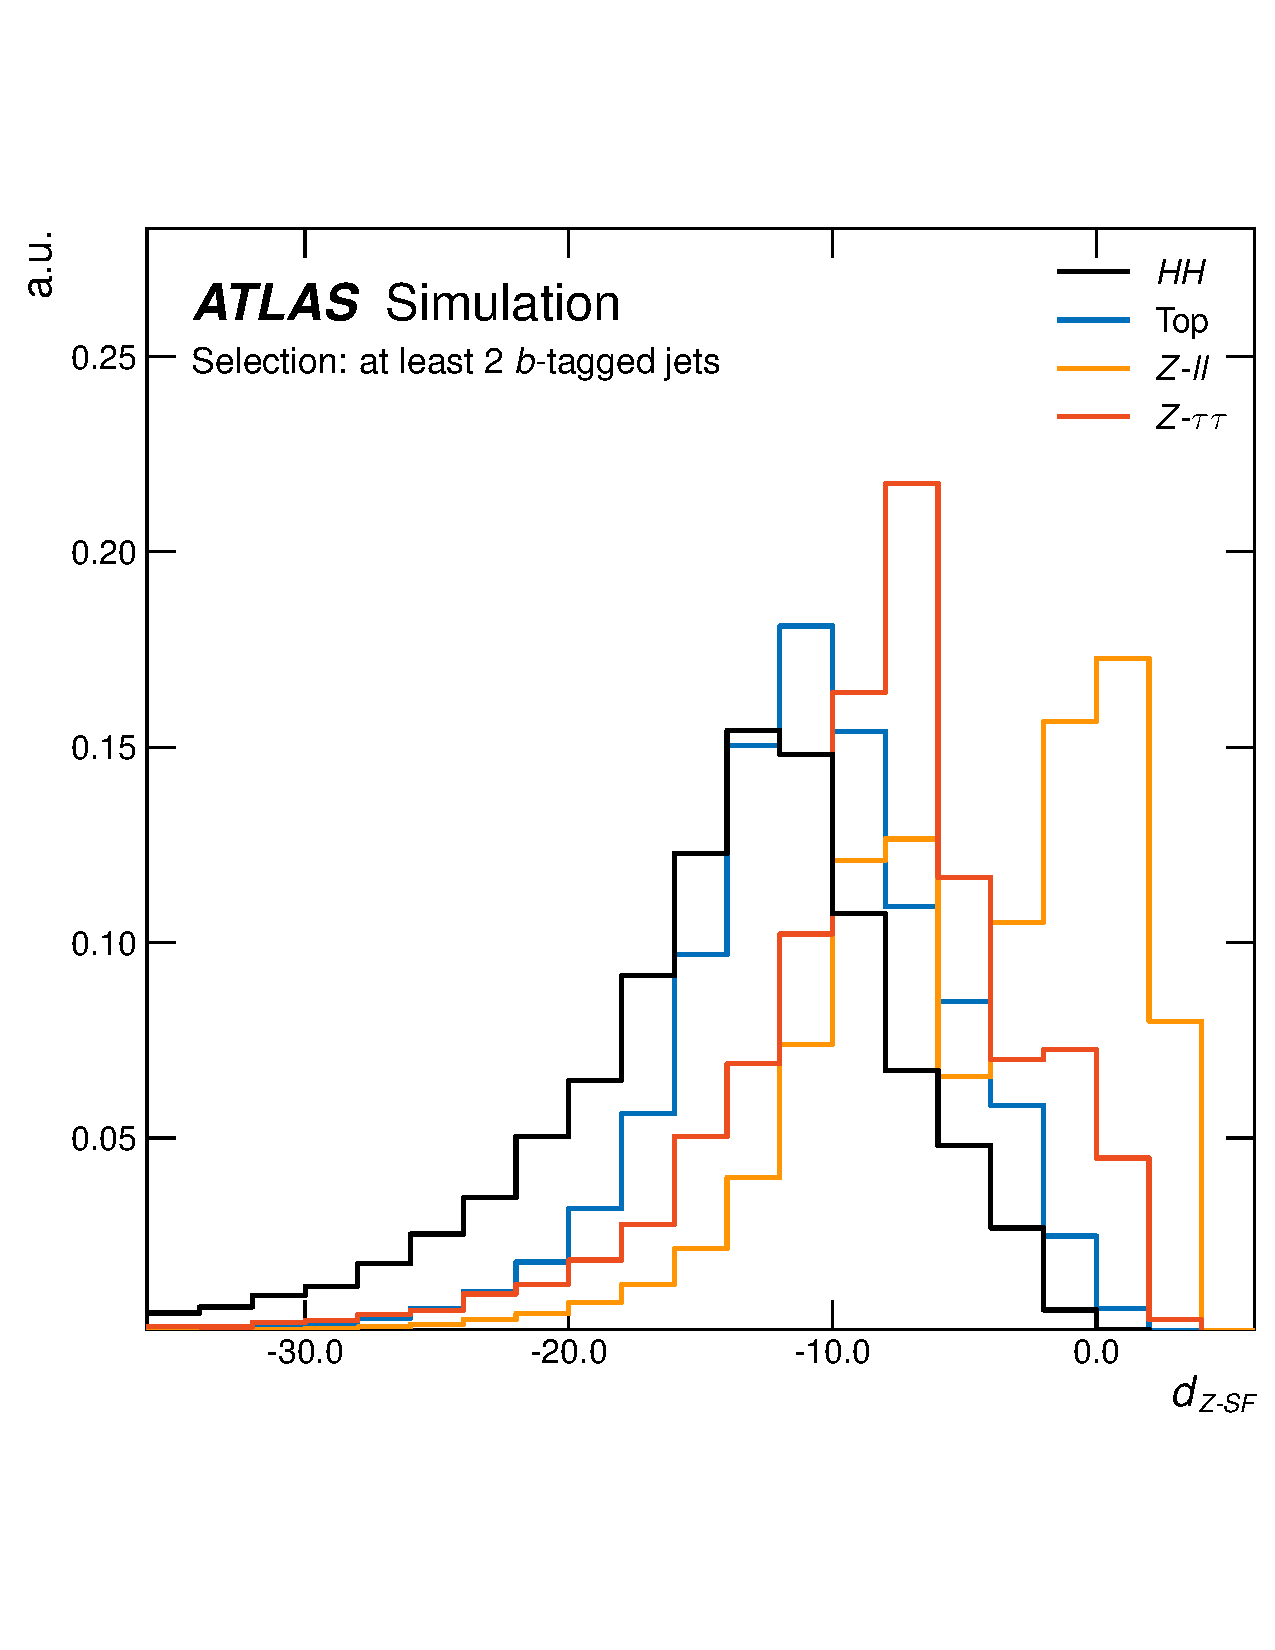
\includegraphics[width=0.48\textwidth]{figures/search_hh/nn_disc/pi_plot_NN_d_zsf}
        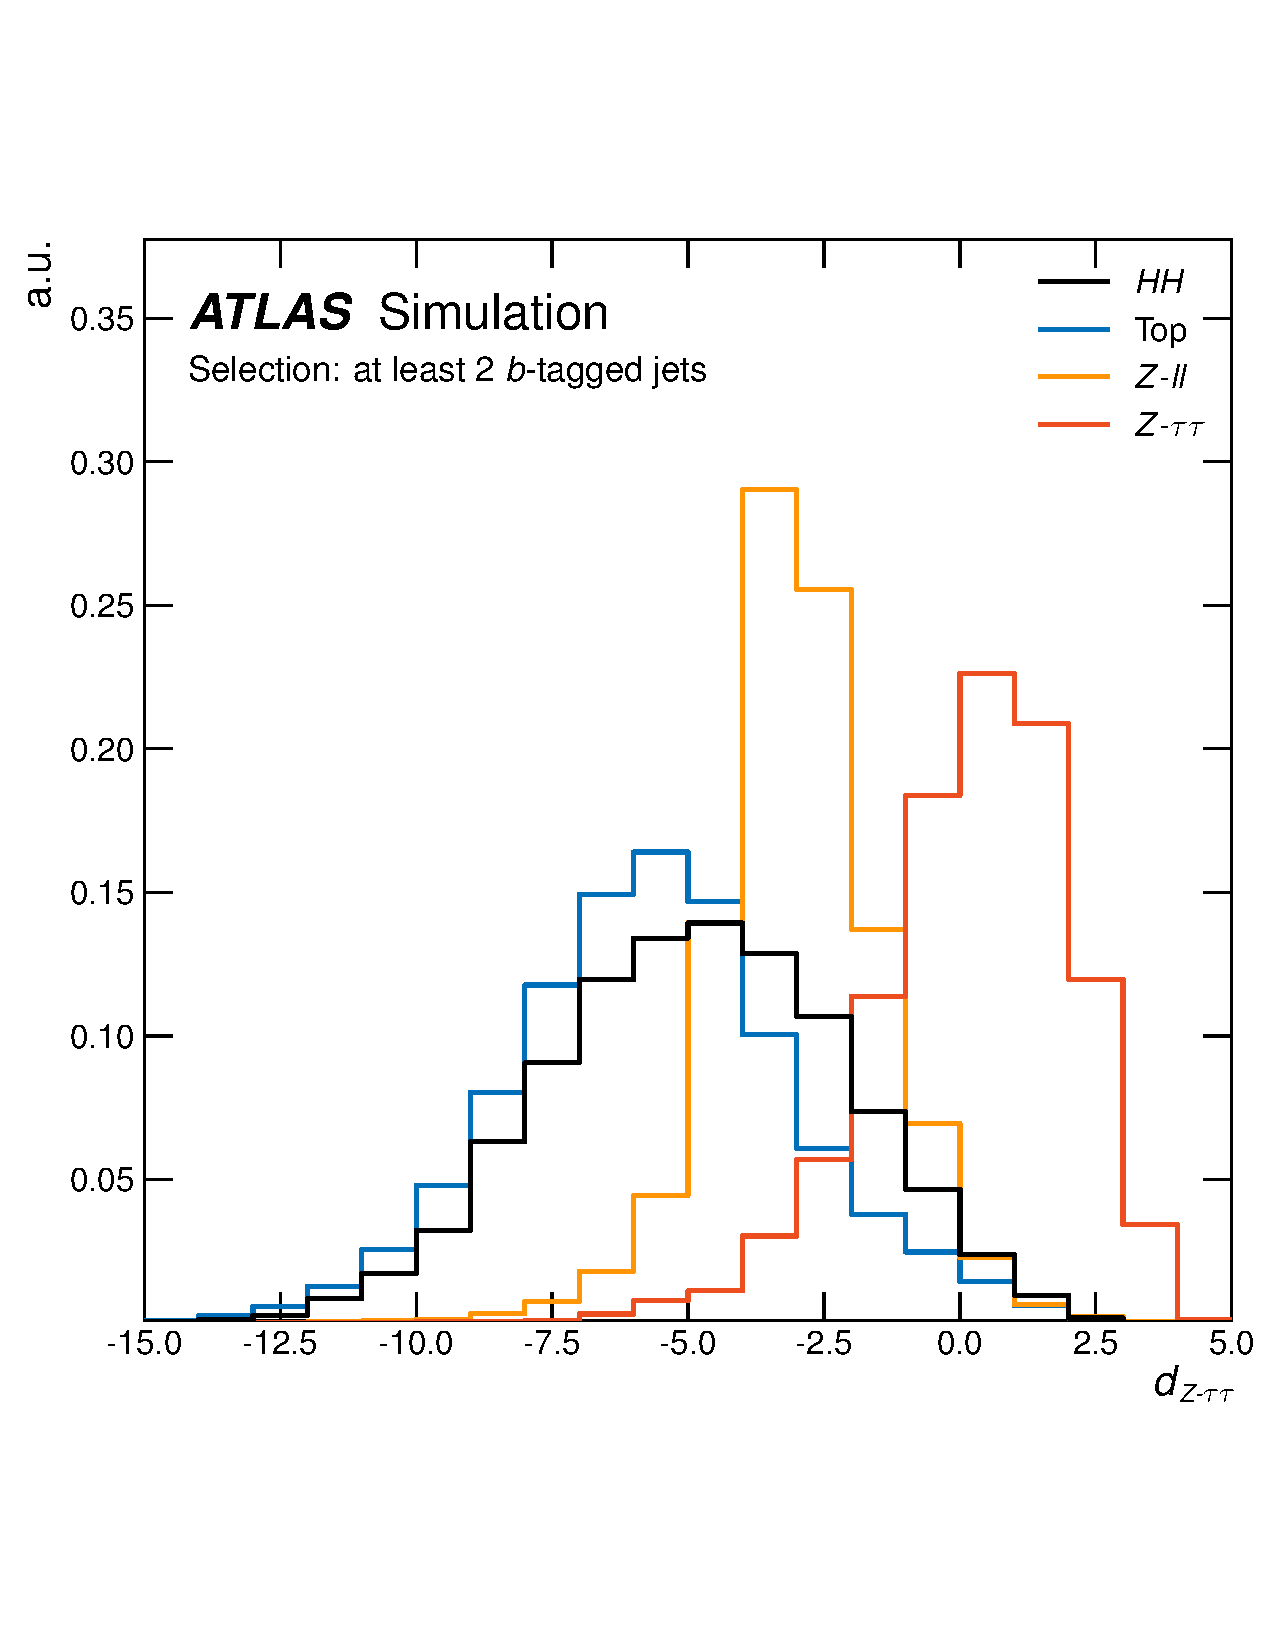
\includegraphics[width=0.48\textwidth]{figures/search_hh/nn_disc/pi_plot_NN_d_ztt}
        \caption{
            Normalized distributions of the four composite discriminants,
            shown for the dilepton
            $hh \rightarrow \bbww$ signal (black), Top (blue), $Z \rightarrow \{ee,\mu\mu\}$ (yellow),
            and $Z\rightarrow \tau\tau$ (orange) processes.
            From the top left and moving clock-wise: \dhh, \dtop, \dztt, and \dzsf.
        }
        \label{fig:nn_disc_d}
    \end{center}
\end{figure}

%%%%%%%%%%%%%%%%%%%%%%%%%%%%%%%%%%%%%%%%%%%%%%%%%%%%%%%%%%%%%%%%%%%%%%%%%%%%%%%%%%%
%%%%%%%%%%%%%%%%%%%%%%%%%%%%%%%%%%%%%%%%%%%%%%%%%%%%%%%%%%%%%%%%%%%%%%%%%%%%%%%%%%%
%%%%%%%%%%%%%%%%%%%%%%%%%%%%%%%%%%%%%%%%%%%%%%%%%%%%%%%%%%%%%%%%%%%%%%%%%%%%%%%%%%%
%
% SR DEFINITION
%
%%%%%%%%%%%%%%%%%%%%%%%%%%%%%%%%%%%%%%%%%%%%%%%%%%%%%%%%%%%%%%%%%%%%%%%%%%%%%%%%%%%
%%%%%%%%%%%%%%%%%%%%%%%%%%%%%%%%%%%%%%%%%%%%%%%%%%%%%%%%%%%%%%%%%%%%%%%%%%%%%%%%%%%
%%%%%%%%%%%%%%%%%%%%%%%%%%%%%%%%%%%%%%%%%%%%%%%%%%%%%%%%%%%%%%%%%%%%%%%%%%%%%%%%%%%

\subsection{Signal Region Definition}
\label{sec:hh_sr_def}

The definitions of the SRs, SR-SF and SR-DF, targeting the dilepton $hh \rightarrow \bbww$ signal process are tabulated
in Table~\ref{tab:hh_sr_def} and are as follows.
The dominant expected backgrounds in the analysis are those for which separate output labels
have been defined in the construction of the neural network classifier described in the previous sections:
SM top-quark processes (\ttbar~and single-top $Wt$) and $Z$+jets processes.
The top-quark processes are flavor symmetric, however the $Z$+jets processes tend primarily to populate
only the same-flavor dilepton final states, with a smaller component in the different-flavor dilepton
final state due to the leptonic $\tau$ decays in the $Z\rightarrow \tau \tau$ process.
For this reason, we define two classes of SR: one requiring SF dilepton events and the
other requiring DF dilepton events.
The SR events are additionally required to have at least two $b$-tagged jets, with
the invariant mass of the two leading $b$-tagged jets having an invariant mass consistent with the
mass of the Higgs boson, $m_{bb} \in [110, 140]$ GeV.
Taking advantage of the lepton correlations, illustrated by Figure~\ref{fig:hh_kin_1},
we further require that the dilepton invariant mass of the SR events be relatively low: $m_{\ell \ell} < 60$ GeV.
This requirement on $m_{\ell \ell}$ effectively acts to remove the majority of background events
arising from $Z$-boson processes.

The SR definitions further rely on placing a cut on the $d_{hh}$ discriminant.
The specific choice of cut, in both SR-SF and SR-DF, are determined by computing the expected 95\% CL cross-section upper-limit
with the selections described in the previous paragraph applied while scanning over varying selections
made on the $d_{hh}$ discriminant.
The cut thresholds on the $d_{hh}$ discriminant in both SR-SF and SR-DF that minimize the cross-section
upper-limit value are chosen as the final values to define SR-SF and SR-DF, and are indicated in Table~\ref{tab:hh_sr_def}.


\begin{table}[!htb]
    \begin{center}
        \caption{
            SRs for the search for the dilepton $hh \rightarrow \bbww$ process.
        }
        \label{tab:hh_sr_def}
        \begin{tabular}{l | c c}
        \hline
        \hline
                & \multicolumn{2}{c}{\textbf{Region}} \\
            \cline{2-3}
            \textbf{Observable} & \textbf{SR-SF} & \textbf{SR-DF} \\
            \hline
            Dilepton Flavor & $ee$ or $\mu\mu$ & $e\mu$ or $\mu e$ \\
            $b$-tagged jet multiplicity & $\ge 2$ & $\ge 2 $ \\
            $bb$-system invariant mass, $m_{bb}$ [GeV] & $\in [110, 140]$ & $\in [110, 140]$ \\
            Dilepton invariant mass, $m_{\ell \ell}$ [GeV] & $<60$ & $<60$ \\
            \dhh & $>5.45$ & $>5.55$ \\
        \hline
        \hline
        \end{tabular}
    \end{center}
\end{table}
